\documentclass[11pt,letterpaper]{article}
\usepackage[utf8]{inputenc}
\usepackage[T1]{fontenc}
\usepackage[spanish]{babel}
\usepackage{amsmath}
\usepackage{amsfonts}
\usepackage{amssymb}
\usepackage{graphicx}
\usepackage{lmodern}
\usepackage{xspace}
\usepackage{multicol}
\usepackage{hyperref}
\usepackage{float}
\usepackage{hyperref}
\usepackage{color}
\usepackage{framed}

\usepackage[left=2cm,right=2cm,top=2cm,bottom=2cm]{geometry}

\newcommand{\X}{\mathbb{X}}
\newcommand{\x}{\mathbf{x}}
\newcommand{\Y}{\mathbf{Y}}
\newcommand{\y}{\mathbf{y}}
\newcommand{\xbarn}{\bar{x}_n}
\newcommand{\ybarn}{\bar{y}_n}
\newcommand{\paren}[1]{\left( #1 \right)}
\newcommand{\llaves}[1]{\left\lbrace #1 \right\rbrace}
\newcommand{\barra}{\,\vert\,}
\newcommand{\mP}{\mathbb{P}}
\newcommand{\mE}{\mathbb{E}}
\newcommand{\mR}{\mathbb{R}}
\newcommand{\mJ}{\mathbf{J}}
\newcommand{\mX}{\mathbf{X}}
\newcommand{\mS}{\mathbf{S}}
\newcommand{\mA}{\mathbf{A}}
\newcommand{\unos}{\boldsymbol{1}}
\newcommand{\xbarnv}{\bar{\mathbf{x}}_n}
\newcommand{\abs}[1]{\left\vert #1 \right\vert}
\newcommand{\muv}{\boldsymbol{\mu}}
\newcommand{\mcov}{\boldsymbol{\Sigma}}
\newcommand{\vbet}{\boldsymbol{\beta}}
\newcommand{\veps}{\boldsymbol{\epsilon}}
\newcommand{\mcC}{\mathcal{C}}
\newcommand{\mcR}{\mathcal{R}}
\newcommand{\mcN}{\mathcal{N}}

\newcommand{\ceros}{\boldsymbol{0}}
\newcommand{\mH}{\mathbf{H}}
\newcommand{\ve}{\mathbf{e}}
\newcommand{\avec}{\mathbf{a}}
\newcommand{\res}{\textbf{RESPUESTA}\\}

\newcommand{\defi}[3]{\textbf{Definición:#3}}
\newcommand{\fin}{$\blacksquare.$}
\newcommand{\finf}{\blacksquare.}
\newcommand{\tr}{\text{tr}}
\newcommand*{\temp}{\multicolumn{1}{r|}{}}

\newcommand{\grstep}[2][\relax]{%
   \ensuremath{\mathrel{
       {\mathop{\longrightarrow}\limits^{#2\mathstrut}_{
                                     \begin{subarray}{l} #1 \end{subarray}}}}}}
\newcommand{\swap}{\leftrightarrow}

\newcommand{\gen}{\text{gen}}
\newtheorem{thmt}{Teorema:}
\newtheorem{thmd}{Definición:}
\newtheorem{thml}{Lema:}
\newtheorem{thme}{Ejemplo:}


\begin{document}
\begin{table}[ht]
\centering
\begin{tabular}{c}
\textbf{Comparaciones múltiples desde la perspectiva de ciencia de datos y}\\
\textbf{su relación con el False Discovery Rate.}\\
\textit{Reporte FDR: Enrique Santibáñez Cortés}
\end{tabular}
\end{table}
\section{False Discovery Rate}
La tasa de falsos descubrimiento (FDR) fue propuesto por primera en Benjamini and Hochberg [1995], la cual se colocó como una de las piezas clave en la investigación relacionada con FDR. Lo anterior debido a que, hasta antes de dicha publicación, la mayor parte de la inferencia relacionada con PHM se hacía fundamentalmente con base en métodos relacionados con el control de FWER, o bien técnicas similares derivadas de modificaciones a la misma. FWER posee desventajas importantes que con el surgimiento de conjuntos de datos de mayor tamaño, por ejemplo en el contexto de genética, se hicieron más evidentes.\\
Esta tasa cambió el panorama de los test de hipótesis multiples, ya que incentivó el desarrollo de numerosas nuevas investigaciones centradas tanto en la búsqueda de nuevas tasas de error derivadas de (\ref{e_fdr}), así como de procedimientos alternativos, al propuesto por BH, para controlar la FDR.\\

La $FDR$  la proporción esperada de errores entre la hipótesis rechazadas. Formalmente, si definimos la variable aleatoria $Q$ como:
\begin{align} \label{e_fdr}
Q=\left\{ \begin{array}{cc}
V/R & R>0\\
0 & R=0
\end{array} \right.
\end{align}
Entonces, se tiene que 
\begin{align*}
FDR = \mE(Q)=\mE\left( \frac{V}{V+S}\right)=\mE\left( \frac{V}{R} \right).
\end{align*}
Por como esta definido $Q$, tenemos que 
\begin{align}\label{igudaldad_Q}
FDR=\mE\left( \frac{V}{R} \right) &= \mE\left( \frac{V}{R}\left| R>0\right. \right)\mP(R>0)+\mE\left( \frac{V}{R}\left| R=0\right. \right)\mP(R=0)\\
&= \mE\left( \frac{V}{R}\left| R>0\right. \right)\mP(R>0).
\end{align}
La tasa $FDR$ tiene propiedades que se relaciona con la tasa $FWER$, algunas son
\begin{enumerate}
\item Si todas las hipótesis nulas son verdaderas, entonces controlar la FDR es equivalente a controlar la FWER. \\
\textbf{Demostración.} Si todas las hipótesis nulas son verdaderas entonces $V=R$. Si $V=0$ entonces $\frac{V}{R}=0$ y si $V>0$ entonces $\frac{V}{R}=1$, por lo que (utilizando el resultado de (\ref{igudaldad_Q}))
\begin{align*}
FDR &= \mE\left( \frac{V}{R}\left| V=0\right. \right)\mP(V=0)+\mE\left( \frac{V}{R}\left| V>0\right. \right)\mP(V>0)\\
&=0\times \mP(V=0)+1\times \mP(V\geq 1)\\
&= \mP(V\geq 1)\\
&= FWER.\ \ \finf
\end{align*}

\item  Si controlamos el FDR (es decir, lo mantenemos por debajo de algún valor), entonces estamos controlando el FWER en el sentido débil. \\
\textbf{Demostración.} Si no todas las hipótesis nulas son verdaderas, entonces $V<R$ y  $\frac{V}{R}<1$, y esto implica que $\mE\left( \frac{V}{R} |V\geq 1\right)<1$. Ocupando lo anterior tenemos
\begin{align*}
FDR&= \mE\left( \frac{V}{R}\left| V=0\right. \right)\mP(V=0)+\mE\left( \frac{V}{R}\left| V\geq 1\right. \right)\mP(V\geq 1)\\
&=0\times \mP(V=0)+\mE\left( \frac{V}{R}\left| V\geq 1\right. \right)\mP(V\geq 1)\\
&<FWER.\ \ \finf
\end{align*}

\end{enumerate}
El punto 2 es el más interesante, pues significa que cualquier procedimiento que controle la FWER también controla la FDR, pero no necesariamente al revés. Decimos por tanto que los procedimientos para el control FWER resultan ser más conservativos, en el sentido de que rechazan en promedio un menor número de hipótesis, que los procedimientos que controlan a FDR. 
\subsection{Procedimiento de control de la FDR de Benjamini y Hochberg(B-H))}
Considere la pruebas $H_1, H_2, ..., H_m$, basado en los p$-$values correspondientes $P_{(1)}, P_{(2)},..., P_{(m)}$. Sean $P_{(1)}\leq P_{(2)}\leq \cdots \leq  P_{(m)}$ los p$-$values están ordenados y denotar por la hipótesis nula $H_{(i)}$ correspondiente a $P_{(i)}$. Defina el siguiente procedimiento de prueba múltiple de Bonferroni$-$type:\\
\begin{align}
 \text{sea k la $i$ más grande para la cual }P_{(i)}\leq \frac{i}{m}q*;\\
 \text{luego rechaza todo }H_{(i)} = 1, 2, ..., k.
\end{align} 

\begin{framed}
    \begin{thmt} \label{t_1}
Para estadísticas de prueba independientes y para cualquier configuración de hipótesis nulas falsas, el procedimiento anterior controla el FDR en $q*$.
    \end{thmt}
\end{framed}
Prueba. El teorema se deriva del siguiente lema, cuya demostración se da en el apéndice A.

\begin{framed}
    \begin{thml} \label{l_1}
Para cualquier $0 <m_0 <m$ p-values independientes correspondientes a hipótesis nulas verdaderas, y para cualquier valor que puedan tomar los p-values de $m_1= m - m_0$ correspondientes a las hipótesis nulas falsas, el procedimiento de prueba múltiple definido por el procedimiento$(1)$ anterior satisface la desigualdad
\begin{equation}\label{2}
\mE (Q | P_{m_0+1}=p_1, ..., P_m = p_{m_1})\leq \frac{m_0}{m} q *
\end{equation}
Ahora, suponga que $m_1=m-m_0$ algunas de las hipótesis son falsas. Cualquiera que sea la distribución conjunta de $P_1'' ,\cdots, P_{m_1}''$, que corresponde a estas falsas hipótesis, integrando la desigualdad (\ref{2}) anterior obtenemos
\begin{equation*}
\mE(Q) <\frac{m_0}{m}q* <q *,
\end{equation*}
y el FDR está controlado.
    \end{thml}
\end{framed}
\textbf{Demostración del lema \ref{2}}. La prueba del lema es por inducción en $m$. Para el caso $m=1$ es inmediato, procedemos asumiendo que el lema es verdadero para cualquier $m'\leq m$, y demostremos que es válido para $m+1$. \\
Si $m_0$ es 0, todas las hipótesis nulas son falsas, por lo que $Q=0$ y 
\begin{align*}
\mE(Q|P_1=p_1,\cdots, P_m=p_m)=0 \leq \frac{m_0}{m+1}q*.
\end{align*} 
Si $m_0>0$, denotemos por $P_i, \ \ i=1,2,\cdots, m_0$ los valores $p$ correspondientes a las verdaderas hipótesis nulas y el mayor de estas $P_{(m_0)}'$. Estos son v.a. independientes $U(0,1)$. Para facilitar la notación asumamos que los $m_1$ p$-$values las hipótesis nulas falsas ordenadas, es decir, $p_1\leq p_2 \leq \cdots \leq p_{m_1}$ y denotemos a $j_0$ más grande de $m_1$ es decir $0\leq j\leq m_1$ que satisface
\begin{align*}\label{desigualdad}
p_j\leq \frac{m_0+j}{m+1}q*,
\end{align*}
y denotemos lo que esta a la derecha de la desigualdad (\ref{desigualdad}) por $p''$, es decir, $$p''=\frac{m_0+j}{m+1}q*.$$
Ahora, condicionando en (\ref{desigualdad}) $P_{(m0)}'=p$ tenemos que 
\begin{align}
\mE (Q | P_{m_0+1}=p_1, ..., P_m = p_{m_1})&=\int_0^1 \mE (Q | P_{(m0)}'=p, P_{m_0+1}=p_1, ..., P_m = p_{m_1}) f_{P_{(m_0)}}'(p)dp\\
&=\int_0^{p''} \mE (Q | P_{(m0)}'=p, P_{m_0+1}=p_1, ..., P_m = p_{m_1}) f_{P_{(m_0)}}'(p)dp+\\
&\int_{p''}^1 \mE (Q | P_{(m0)}'=p, P_{m_0+1}=p_1, ..., P_m = p_{m_1}) f_{P_{(m_0)}}'(p)dp
\end{align} 
donde $f_{P_{m_0}}=m_0p^{(m_0-1)}.$
Para la primera parte cuando $p\leq p''$. Como todas las hipótesis $m_0+j_0$ nulas son rechazadas, y $Q=m_0/(m_0+j_0)$. Entonces evaluando la primera integral, y usando (\ref{desigualdad})
\begin{align}\label{desigualdad_6}
\frac{m_0}{m_0+j_0}(p'')^{m_0} \leq \frac{m_0}{m_0+j_0} \frac{m_0+j_0}{m+1}q*(p'')^{m_0-1}=\frac{m_0}{m+1}q*(p'')^{m_0-1}.
\end{align}

Ahora, en la segunda parte de la integral (--), consideremos separar cada $p_{j_0}< p_j\leq P_{(m_0)}'=p<p_{j+1}$ y $p_{j_0}< p'' \leq P_{(m_0)}'=p<p_{j_0+1}$.  Es importante señalar que, debido a la forma en que se definen $j_0$ y $p"$, no se puede rechazar ninguna hipótesis como resultado de los valores de $p, p_{j + 1}, p_{j + 2},\cdots, p_{m_1}$. Por lo tanto, cuando todas las hipótesis son verdaderas y falsas se consideran juntas, y sus valores $p$ así ordenados, una hipótesis $H_{(i)}$ puede rechazarse solo si existe $k, i <k<m_0 + j-1$, para lo cual $p_{(k)} <\{k / ( m + 1)\} q *$, o equivalentemente 
\begin{align}\label{q_p_k}
\frac{p_{(k)}}{p}\leq \frac{k}{m_0+j-1} \frac{m_0+j-1}{(m+1)p}q^*.
\end{align}
Cuando se condiciona con $P_{(m_0)}'=p$, los $P_j'/p$ para $i=1,2, \cdots, m_0-1$ son $m_0-1$ v.a's independientes con distribución $U(0,1)$. y los $p_i/p$ para $i=1,2, \cdots,j$ corresponden al número de hipótesis nulas falsas entre 0 y 1. 
Usando la desigualdad (\ref{q_p_k}) para las $m_0+j-1=m'\leq $ hipótesis es equivalente usando que $P_{(i)}\leq \frac{i}{m}q*$, con cota $\{(m_0+j-1)/(m+1)p \}q*$. Aplicando ahora la hipótesis de inducción tenemos que 
\begin{align}\label{final}
\mE (Q | P_{(m0)}'=p, P_{m_0+1}=p_1, ..., P_m = p_{m_1}) \leq \frac{m_0-1}{m_0+j-1} \frac{m_0+j-1}{(m+1)p}q^* = \frac{m_0-1}{(m+1)p}q^*.
\end{align}
Considerando la desigualdad (\ref{final}) depende de $p$, pero no del segmento $p_j<p<p_{j+1}$ ppr lo cuál podemos integral y ocupando (\ref{desigualdad_6}) podemos concluir que 
\begin{align*}
\int_{p''}^1\mE (Q | P_{(m0)}'&=p, P_{m_0+1}=p_1, ..., P_m = p_{m_1})f_{P_{m_0}}'(p) \leq  \frac{m_0-1}{(m+1)p}q^*m_0p^{(m_0-1)}dp\\
&=\frac{m_0}{m+1}q*\int_{p''}^1(m_0-1)p^{(m_0-2)}dp=\frac{m_0}{m+1}q^*\{1-p''^{(m_0-1)} \}. \ \ \finf
\end{align*}

Cabe aclarar que una de las principales desventajas potenciales del algoritmo B-H tal y como se propuso en Benjamini and Hochberg [1995] yace en el supuesto de independencia entre las m hipótesis requerido para asegurar el control de la FDR. En respuesta a esa situación Benjamini and Yekutieli [2001] demuestran que el procedimiento B-H también puede ofrecer control de la FDR para los casos en los cuales las hipótesis están positivamente correlacionadas, como es el caso en una gran variedad de aplicaciones como en Génetica y Ecología. 

\subsection{Ejemplos de control}

\subsubsection*{Comparación de la FDR y FWER}
Se ha demostrado que la trombólisis con activador de plasminógeno de tipo tisular recombinante ($rt-PA)$ y activador de estreptoquinasa de plasminógeno anisoilado (APSAC) en el infarto de miocardio reduce la mortalidad. Neuhaus y col. (1992) investigaron los efectos de una nueva administración de carga frontal de rt$-$PA versus los obtenidos con un régimen estándar de APSAC. El estudio se pueden identificar cuatro familias de hipótesis, pero la que puede ser deseable el control de FDR ya que no se quiere concluir que el tratamiento de carga frontal sea mejor si es simplemente equivalente al tratamiento anterior en todos los aspectos es en las pruebas: en eventos cardíacos y de otro tipo después del inicio del tratamiento trombolítico (15 hipótesis).

Los p$-$values individuales se informan tal como están, sin advertencia alguna sobre su interpretación y los autores concluyen que\\

''\textit{En comparación con el tratamiento con APSAC, a pesar de más reoclusiones tempranas, el curso clínico con el tratamiento con rt-PA es más favorable con menos complicaciones hemorrágicas y una tasa de mortalidad hospitalaria sustancialmente más baja, presumiblemente debido a una mejor permeabilidad temprana de la arteria relacionada con el infarto}''.\\

La afirmación sobre la mortalidad se basa en un valor de p de 0,0095.\\ Considere ahora la cuarta familia, que contiene la comparación de mortalidad y otras 14 comparaciones. Las posiciones ordenadas para las 15 comparaciones realizadas son \begin{align*}
0001, 0,0004, 0,0019, 0,0095, 0,0201, 0,0278, 0,0298,\\ 0,0344, 0.0459, 0.3240, 0.4262, 0.5719, 0.6528, 0.7590, 1.000.
\end{align*}
Controlando el FWER en 0.05, el enfoque de Bonferroni, usando $0.05 / 15 = 0.0033$ rechazamos las tres hipótesis correspondientes a los valores $p$ más pequeños (ver cuadro \ref{t_p_ejecicio}). Y usando el procedimiento de control de FDR considerando el enfoque $BH$ con $q^* = 0.05$ rechazamos las cuatro hipótesis que tienen valores $p$ menores o iguales a $0.013$.

\begin{table}[H] \label{t_p_ejecicio}
\begin{tabular}{ccccccccccc}
\hline
\hline
$H_{0i}$ & p$-$values & i &  Umbral BH & Umbral Bonferroni & Rechazo BH& Rechazo Bonferroni\\
\hline
\hline
1 &   0.0001&  1& 0.0034&       0.0033&       TRUE&               TRUE\\
2 &   0.0004&  2& 0.0067&       0.0033&       TRUE&               TRUE\\
3 &   0.0019&  3& 0.0100&       0.0033&       TRUE&               TRUE\\
4 &   0.0095&  4& 0.0134&       0.0033&       TRUE&              FALSE\\
5 &   0.0201&  5& 0.0167&       0.0033&      FALSE&              FALSE\\
6 &   0.0278&  6& 0.0200&       0.0033&      FALSE&              FALSE\\
7 &   0.0298&  7& 0.0234&       0.0033&      FALSE&              FALSE\\
8 &   0.0344&  8& 0.0267&       0.0033&      FALSE&              FALSE\\
9 &   0.0459&  9& 0.0300&       0.0033&      FALSE&              FALSE\\
10&   0.3240& 10& 0.0334&       0.0033&      FALSE&              FALSE\\
11&   0.4262& 11& 0.0367&       0.0033&      FALSE&              FALSE\\
12&   0.5719& 12& 0.0400&       0.0033&      FALSE&              FALSE\\
13&   0.6528& 13& 0.0434&       0.0033&      FALSE&              FALSE\\
14&   0.7590& 14& 0.0467&       0.0033&      FALSE&              FALSE\\
15&   1.0000& 15& 0.0500&       0.0033&      FALSE&              FALSE\\
\hline
\hline
\end{tabular}
\caption{Resultados de los p$-$values.}
\end{table}

Las primeras tres hipótesis corresponden a una reacción alérgica reducida y a dos aspectos diferentes del sangrado; no incluyen la comparación de mortalidad. Por tanto, la afirmación sobre una reducción significativa de la mortalidad no está justificada desde el punto de vista clásico. Pero controlando el FDR rechazamos la hipótesis 4,  ahora con la confianza apropiada las afirmaciones sobre la disminución de la mortalidad, de las que antes no teníamos pruebas suficientemente sólidas.\\

En la figura  (\ref{comparacion_métodos}) observamos los umbrales rechazar la hipótesis nula  para las distintas metodologías. Se observa claramente que las metodologías para controlar el $FWER$ resultan más conservativas ya que tiene un umbral muy pequeño para rechazo, en cambio si se controla el $FDR$ el umbral es 0.5.

\begin{figure}[H]
\centering \label{comparacion_métodos}
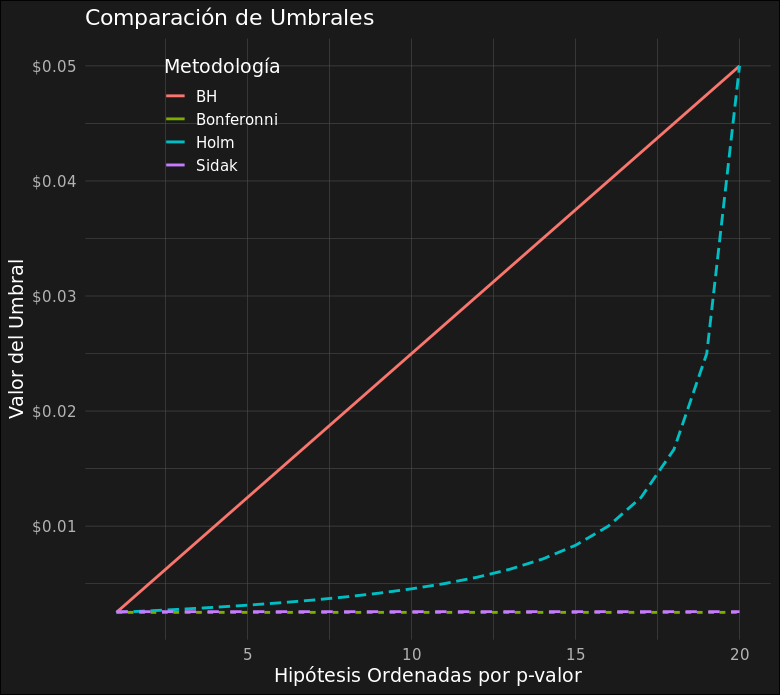
\includegraphics[scale=.5]{comparacion_de_metodos.png}
\caption{Comparación del valor del Umbral de rechazo}
\end{figure}

\subsection*{Aplicación del FDR en la ciencia de datos}
\subsubsection*{Análisis de ejemplo: Enfermedades relacionadas con la edad influyen en la morfología cerebral}

En este ejemplo, se realizó un análisis de las masas en imágenes de resonancia magnética (RM) extraídas de la iniciativa de datos abiertos de la serie de acceso abierto de estudios de imágenes (OASIS). Estos datos contienen imágenes ponderadas en T1 de 416 participantes con y sin demencia de entre 18 y 96 años, lo que permite investigar cómo la edad y las enfermedades relacionadas \textbf{con la edad influyen en la morfología cerebral}.\\

Para descargar el conjunto de datos de OASIS, visite $http://www.oasis-brains.org/\#data$ y elija el lanzamiento OASIS-1, que contiene imágenes de resonancia magnética (MR) de 416 participantes de entre 18 y 96 años. El archivo de información del participante incluye variables demográficas básicas (edad, género, mano de obra, nivel educativo, estatus socioeconómico), variables clínicas y estimaciones de volumen cerebral. 

El objetivo del estudio fue determinar que partes del cerebro están relacionadas de su edad. Para probar este hecho se considero calcular los coeficientes de correlación Spearman  entre el grosor cortical y la edad en cada vóxel cortical, y se consideraron 163810 pruebas de la siguiente forma
\begin{align*}
H_{0i}: \rho_s =0 \ \ \ vs \ \ \ H_{0i}:\rho_s\neq 0, \ \ \forall i=1,\cdots, 163810.
\end{align*}
donde $\rho_s=1-\frac{6\sum d_i^2}{n(n^2-1)}$ y $d_i=rg(X_i)-rg(Y_i)$ es la diferencia de los rangos de cada observación. Se puede probar que si $n$ es grande entonces (basado en un argumento de permutación) 
$$\rho_s\sqrt{\frac{n-2}{1-\rho_s^2}} \sim t_{n-2}$$.
Por lo que es sencillo probar significancia con lo anterior. Por lo tanto, considerando lo anterior procedió a calcular los p$-$values de cada juego de hipótesis. Y posterior se le aplicaron las correcciones de Sidák para controlar el family$-$wise error rate (FWER), y el procedimiento BH para controlar la FDR. 
\begin{figure}[H]
\centering \label{cerebro}
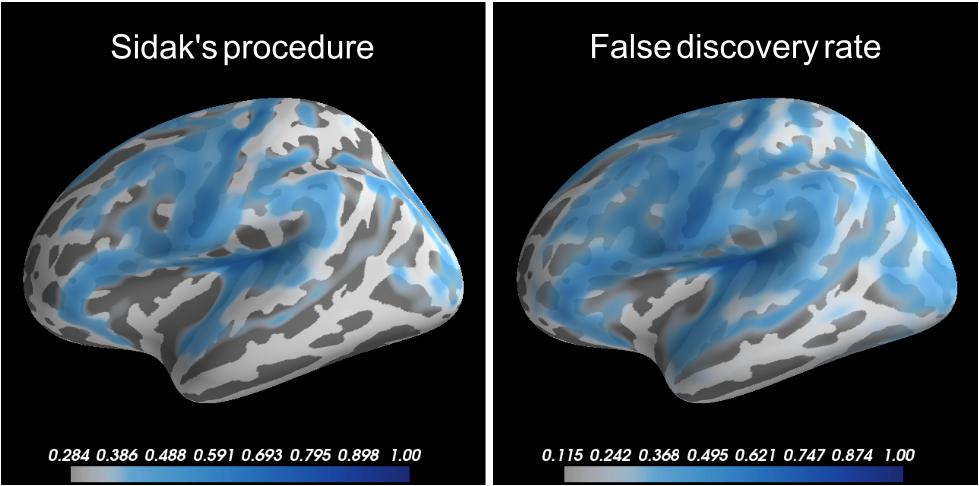
\includegraphics[scale=.5]{neurociencia_FDR_FWER.png}
\caption{Diferencias cuando se controla el FWER y el FDR.}
\end{figure}
Un total del $55\%$ de los vóxel mostró un efecto estadísticamente significativo del envejecimiento sobre el grosor cortical cuando los valores p se corrigieron para múltiples pruebas usando la corrección de Sidak. Por el contrario, cuando la corrección se basó en el procedimiento Benjamini-Hochberg FDR, el número de vértices significativos fue del $82\%$, lo que sugiere un efecto más generalizado. El nivel crítico sin corregir se fijó en $\alpha = 0.05$ en ambos análisis.
Los resultados se muestran en la figura (\ref{cerebro}), lo cuál podemos concluir que algunos de los mayores efectos relacionados con la edad se observan en el surco central.
\subsubsection*{FDR en la selección del modelo.}
La selección hacia adelante es un tipo de regresión por pasos que comienza con un modelo vacío y agrega variables una por una. En cada paso hacia adelante, agrega la variable que brinda la mejor mejora individual a su modelo.

\subsubsection*{Controling the False-Discovery Rate in Astrophysical Data Analysis.} 

'\textit{El propósito de este artículo es presentar el procedimiento FDR a la comunidad astrofísica. Ilustramos el poder de FDR a través de varios ejemplos astronómicos, incluida la detección de características frente a una función unidimensional suave, por ejemplo, ver las \textit{ondulaciones de bariones} en un espectro de potencia de fluctuaciones de materia y detección de píxeles de origen en datos de imágenes. En esta era de grandes conjuntos de datos y mediciones de alta precisión, FDR proporciona los medios para controlar de manera adaptativa una cantidad cientícamente significativa: la fracción de descubrimientos falsos sobre el total de descubrimientos.}'.

\end{document}